\scanpage{76}
% archive sheet number: 75
\diagram{\(\begin{array}{ll|l}
S_0=(0,0,0)&\underline aS_0=(\alpha',1-\alpha',1-\alpha')&\underline a(x,y,z)=(\alpha'-x,(1-\alpha')-y,(1-\alpha')-z)\\
S_1=(1,0,0)&\underline aS_1=(\alpha'-1,1-\alpha',1-\alpha')&c=\frac12(\alpha',1-\alpha',1-\alpha')\\
S_2=(0,1,0)&\underline aS_2=(\alpha',\unsure{-\alpha'|-\alpha'_2},1-\alpha')&\text{centre}\\
S_3=(0,0,1)&\underline aS_3=(\alpha',1-\alpha',-\alpha')&u=2c=(\alpha',1-\alpha',1-\alpha',2)\\
S'_3=(\alpha',-\alpha',\unsure{2|1})&\underline aS'_3=(0,1\deleted{\unsure{+\alpha'|-\alpha'}},-\alpha')&\\
S''_3=(0,-\alpha',1)&\underline aS''_3=(\alpha',1-2\alpha',-\alpha')&
\end{array}\)}
\[
\begin{aligned}
q_0(x,y,z)&=x^2+y^2+z^2-\alpha yz+\unsure{X|x}(y+z)-(x+y+z)\\
\bigl[&=(\text{en car. }2)\quad\alpha'\bigl[(x-\alpha y)^2+\alpha'(x-\alpha y)(x-\alpha z)+(x-\alpha z)^2\bigr]\\
&\hspace{7em}-(x+y+z)\bigr]
\end{aligned}
\]
Si $e$ est un vecteur arête (tel que $s_1-s_0=e_1$),
\[
f\quad\text{---}\quad\text{coarête}\quad(\text{tel que }s_3-s_2=e_3-e_2)
\]
\[
\left\{\begin{aligned}
q(e)&=1\quad\text{(c'est la normalisation de }q\text{ !)}\\
q(f)&=\alpha+2\\
q(f)/q(e)&=\alpha+2=(\alpha+1)^2=\alpha'^2
\end{aligned}\right.
\]
En coordonnées distinguées, si $(\pm x,\pm y,0),(\deleted{\unsure{+}}\pm y,0,\pm x),(0,\pm x,\pm y)$ sont les $12$ sommets de l'icosaèdre, on aura (si $(x,y,0)$ et $(-x,y,\unsure{0})$ sont les sommets d'une arête, donc $(x,y,0)$ et $(x,-y,0)$ ceux d'une coarête)
\figure{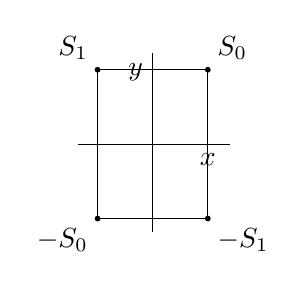
\begin{tikzpicture}[scale=.7]
\draw (-1,-1.35) rectangle (1,1.35);
\draw (0,-1.6)--(0,1.65) (-1.35,0)--(1.4,0);
\fill (-1,1.35) circle (1.5pt);\fill (1,1.35) circle (1.5pt);\fill (-1,-1.35) circle (1.5pt);\fill (1,-1.35) circle (1.5pt);
\node[above left] at (-1,1.35) {$S_1$};\node[above right] at (1,1.35) {$S_0$};\node[below left] at (-1,-1.35) {$-S_0$};\node[below right] at (1,-1.35) {$-S_1$};\node[left] at (0,1.3) {$y$};\node[below] at (1,0) {$x$};
\end{tikzpicture}}
\[
\deleted{\unsure{\frac{4y^2}{4x^2}=\lambda\left(\frac yx\right)^2}}\deleted{\unsure{\alpha}}\frac{q(f)}{q(e)}=\frac{4y^2}{4x^2}=\left(\frac yx\right)^2=\alpha'^2\quad\text{donc}\quad\frac yx=\pm\alpha'
\]
(dans le cas réel, \unsure{l'icosaèdre|d'icosaèdre} convexe, $\alpha=\frac12(-1+\sqrt5)$, $\alpha'=\frac12(-1-\sqrt5)$, \deleted{\unsure{et}} et si on prend $x,y>0$, on trouve $y/x=-\alpha'=\frac12(1+\sqrt5)$)
\[
\delta'(q_0)=1\qquad\text{Matrice }\unsure{\varphi|\phi}_{q_0}=\begin{pmatrix}2&1&1\\1&2&-\alpha\\1&-\alpha&\deleted{\unsure{0}}2\end{pmatrix}
\]
Matrice non singulière sauf en car. $2$, où le noyau de $\varphi_{q_0}$ est engendré par le vecteur $u=(\alpha',1-\alpha',1-\alpha')=(\alpha',\alpha,\alpha)=(1+\alpha,\alpha,\alpha)$ NB $q_0(u)=\alpha'\ne0$, ce qui exprime la \unsure{non-singularité|nonsingularité} de $q_0$ en car. $2$)
